\newpage
\chapter{Word-Vectors}

Word vectors represent a significant leap forward in advancing our ability to analyze relationships across words, sentences, and documents. In doing so, they advance technology by providing machines with much more information about words than has previously been possible using traditional representations of words. It is word vectors that make technologies such as Machine translation, Sentiment analysis, Speech recognition, Question Answering possible.\\

\noindent This chapter will explain the following:
\begin{itemize}
\item{Need for word-embeddings}
\item{History of word-embeddings}
\item{Word-vector training}
\item{Semantic Relationship and similarity}
\item{Word Pairs and Phrases}
\item{Applications of word embeddings}
\item{Current advances in word-embeddings}
\end{itemize}

\section{Need for word-embedding}

Traditional NLP systems treated words as atomic units, such as one-hot encoding and bag-of-words models. These methods used dummy variables to represent the presence or absence of a word in an sentence. For the one-hot encoding, each word is represented by a one-hot vector - a sparse vector in the size of the vocabulary, with 1 representing the presence of a word and 0 representing its absence. The bag-of-words feature vector considers the word occurrence as feature value which is normalized using term frequency and inverse-document frequency to increase the importance of rare words and reduce the importance of very frequent but less important words like stop words.

This choice of word-representation is simple, robust and can act as a good baseline model which can be coded using a few lines of code. It also works very well when your dataset is small and the context is domain specific. However these models do not preserve the semantic relationship between words and hence lose important linguistic patterns such as word-order and synonyms. Ex. "This is good" and "Is this good" have the same feature representation. They are also difficult to model highly sparse data. Thus, simple scaling up of basic techniques will not result in any significant progress, and we have to focus on more advanced techniques.

\section{History of word-embeddings}

The technique of representing words as vectors has roots in the 1960s with the development of vector space models for information retrieval. Reducing the number of dimensions using singular value decompostitoin led to the introduction of latent semantic analysis in the late 1980s. In 2001, Bengio et al. \cite{bengio2003neural} published a paper to tackle language modeling and it was the initial idea of word-embedding. At that time, they named this process as "learning a distributed representaion for words".

In 2008, Ronan and Jason \cite{collobert2008unified} introduced a concept of pre-trained model and showed its amazing approach for solving NLP problems. In 2013, a team at Google led by Tomas Mikolov created word2vec \cite{mikolov2013efficient}, a word-embedding toolkit which can train vector space models faster than the previous approaches. Later on, gensim provided an amazing wrapper so that adopt different pre-trained word-embedding models which include Word2Vec (by Google), GloVe \cite{pennington2014glove} (by Stanford), fastText (by Facebook).

\section{Word-vector training}

Training a word2vec model is similar to an autoencoder. We use a simple neural network with a single hideen layer to perform a certain task, but then we're not going to use it for the task we trained it for. Instead, the goal is to just learn the weights of the hidden layer that are actually the word-vectors that we're trying to learn.

Training the model is done in one of two ways, either using the context to predict a target word (known as continuous bag of words or CBOW) or using a word to predict a target context, which is called skip-gram. According to Mikolov, the skip-gram model works well with small amount of training data and represents well even rare words or phrases. The CBOW is several times faster to train than the skip-gram and shows slightly better accuracy for the frequent words. Let us first look at the skip gram model.

We're going to train the neural network to do the following: Given a specific word in the middle of a sentence (the input word), look at the nearby words and pick one at random. The network is going to predict the probability for every word in the vocabulary of being the nearby word that we choose. The nearby word is actually a window size parameter to the algorithm. A typical window size might be 5.

The output probabilities indicate how likely is it to find each word near our input word. For example, the input word "Soviet" will have higher probabilities for words like "Union" and "Russia" than for unrelated words like "watermelon" and "kangaroo". The neural network will be trained by feeding it word pairs from the train data. The below example shows some of the training samples. The word highlighted in blue is the input word.

\begin{figure}[htbp]
\centering
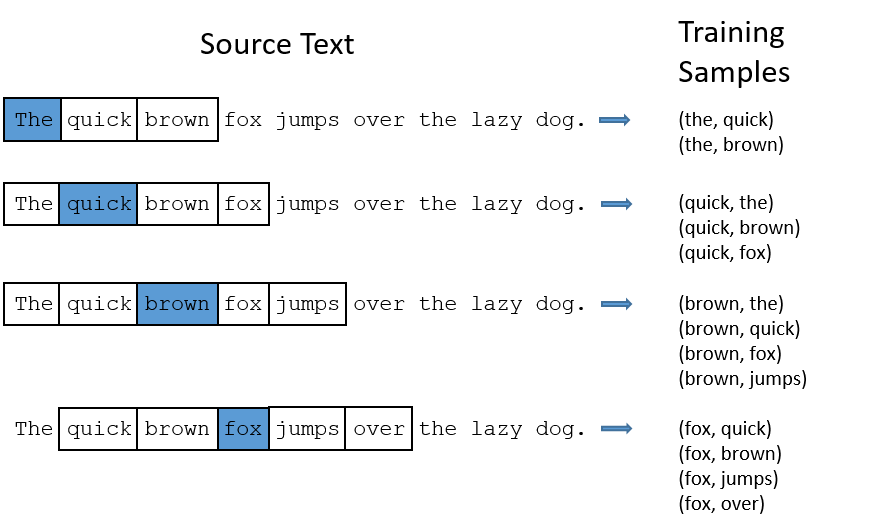
\includegraphics[width=16cm, height=10cm]{images/training_data.png}\\
\centering
\caption{Training samples for skip-gram model having a window size of 2.}
\label{fig:foo}
\end{figure}

\newpage
\subsubsection{Model details}

The words cannot be fed to the neural network as a text string. To do this, we represent the words as a one-hot vector. If we have a vocabulary of 10,000 unique words, then the one-hot vector will have 10,000 components (one for every word in the vocabulary) and we'll place a 1 in the position corresponding to the word and 0 in all other positions. The output of the network is also a single vector with 10,000 components containing the probability that a randomly selected nearby word is that vocabulary word. Thus, the output vector will actually be a probability distribution and not a one-hot vector.

If we want to learn our word-vectors with 300 features, the hidden layer would be represented by a weight matrix with 10,000 rows and 300 columns and the end goal is just to learn the hidden layer weight. The output layer is trained using a softmax regression classifier. The network diagram for both the skip-gram and continuous bag of words models can be seen in the next page.

\begin{figure}[htbp]
\centering
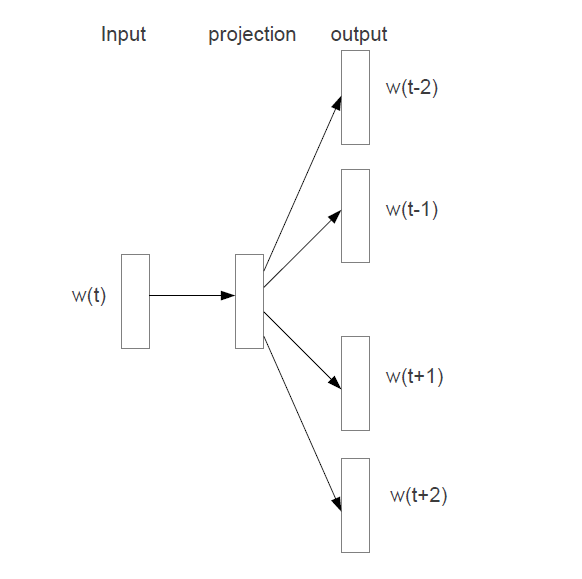
\includegraphics[width=16cm, height=10cm]{images/skip-gram.PNG}\\
\centering
\caption{Skip-gram model: Predicts the surrounding words given the current word.}
\label{fig:foo}
\end{figure}

\begin{figure}[htbp]
\centering
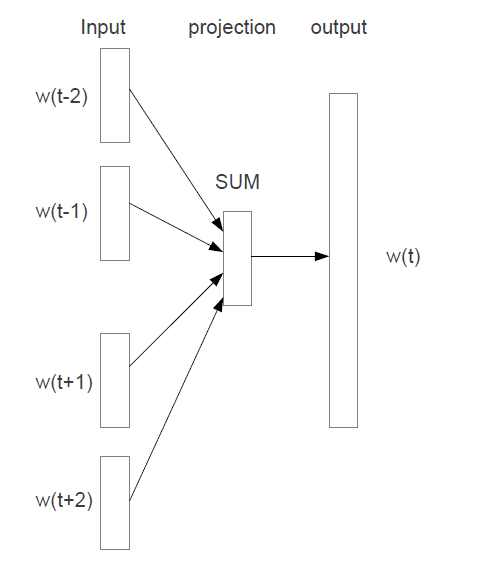
\includegraphics[width=16cm, height=10cm]{images/CBOW.PNG}\\
\centering
\caption{Continuous Bag of words model: Predicts the current word given the context.}
\label{fig:foo}
\end{figure}

\subsubsection{Improvements to the model}

From the previous example, we've seen that for word-vectors with 300 components and 10,000 vocabulary size, both the hidden and output layers will have the weight matrix of size 300 x 10,000 = 3 million weights each. Running gradient descent on a neural network that large is going to be slow. To address this issue, the word2vec authors addressed this issue in their paper with the following two innovations:

\begin{itemize}
\item{subsampling frequent words to decrease the number of training examples}
\item{modifying the optimization objective through "Negative sampling" which causes each training sample to update only a small percentage of model's weights.}\\
\end{itemize}
\noindent\textbf{Subsampling Frequent words:}\\

In the previous example of the sentence, "The quick brown fox jumps over the lazy dog.", we've seen two common problems. Firstly, word pairs like (fox, the) doesn't tell us much about the meaning of "fox" as "the" appears in the context of almost every word. Secondly there are many samples of "the" than needed to learn a good vector for it. To remediate this, word2vec implements a subsampling scheme that subsamples some of the words from the training data based on its frequency.\\

\noindent\textbf{Negative Sampling:}\\

Instead of every training sample tweaking all the weights of the neural network, we can modify only a small percentage of weights, rather than all of them. With negative \cite{goldberg2014word2vec}, we are going to randomly select a small number of negative weights to update along with updating all the positive weights. The negative samples are selected using a unigram distribution, where frequent words are more likely to be selected as negative samples. Thus the probability of picking the word as part of a negative sample to update will depend on the number of times the word appears in the corpus divided by the total number of words in the corpus. This is expressed by the following equation:

\begin{equation}
P(w_{i}) = \frac{f(w_{i})}{\sum_{j=0}^{n}f(w_{j})}
\end{equation}

The word vector space implicitly encodes many regularities among words. The resulting distributed representation of words contain a lot of syntactic and semantic information which we will see in the next section.

\section{Semantic Relationship and Similarity}

Word vectors represent words as a vector of real valued numbers where each point captures a dimension of the word's meaning. Thus, if two different words have very similar "contexts" i.e., what words are likely to appear around them, then the model needs to output very similar results for these two words. And one way for the network to output similar context predictions for these two words is if the word-vectors are similar. So, if two words have similar contexts, then the network will eventually learn similar word vectors for these two words. This means that words such as "engine" and "transmission" should have similar word vectors to the word "car", whereas the word "pineapple" should be quite distant. This can also handle stemming for you - the network will likely learn similar word-vectors for words like "man" and "men" because these should have similar contexts.

\newpage

\begin{figure}[htbp]
\centering
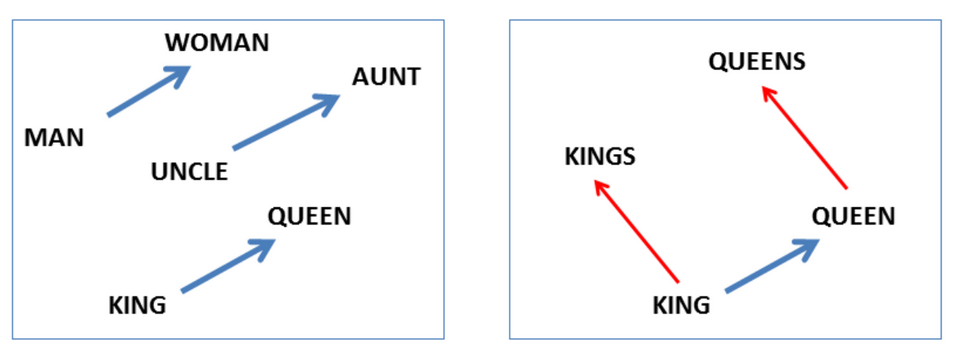
\includegraphics[width=12cm, height=6cm]{images/wv-similarities.PNG}
\centering
\caption{The word vector space encodes many regularities among words.}
\label{fig:foo}
\end{figure}

\noindent \textbf{Analogies:}\\

The famous examples that show incredible properties of embeddings is the concept of analogies. We can add and subtract word embeddings and arrive at interesting results. The most famous example is the formula:
\begin{itemize}
\item{"king" - "man" + "woman" = "queen"}
\end{itemize}
In other words, we can subtract one meaning from the word vector for king (i.e. maleness), add another meaning (femaleness), and show that this new word vector maps closely to the word vector for queen.

\begin{figure}[htbp]
\centering
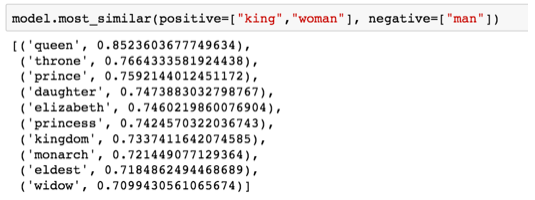
\includegraphics[width=16cm, height=8cm]{images/king-man+woman-gensim.png}\\
\centering
\caption{The image shows that we can add and subtract word vectors and it would find the most similar words to the resulting vector.}
\label{fig:foo}
\end{figure}

\newpage
\section{Word Pairs and Phrases}

The current implementation of word vectors is limited to its unigram natural behavior. It does not embed bigrams like "American Airlines" as its whole. In some cases, a word pair like "Boston Globe" (a newspaper) has a much different meaning than the individual words "Boston" and "Globe". So it makes sense to treat "Boston Globe" as a single term whenever it occurs when its own word vector representation.

However, the addition of phrases to the model will exponentially increase the vocabulary size. The word2vec team have built a tool that counts the number of times each combination of two words appears in the training text, and use it in an equation to determine which word combinations turn into phrases \cite{mikolov2013distributed}. The equation is designed to make phrases out of words which occur together often relative to the number of individual occurrences. It also favors phrases made of infrequent words in order to avoid making phrases out of common words like "and the" or "this is".

The same word2vec idea can be extended to sentences and complete documents where instead of learning feature representation for words, you learn it for sentences or documents. The applications of these models could depend on the task at hand. A word2vec model can effectively capture semantic relationship between words and hence it can be used to calculate word similarities or fed as features to various NLP tasks such as sentiment analysis, LSTMs etc. However words can only capture so much, there are times when you need relationships between sentences and documents and not just words. For example, if you are trying to figure out if two documents are duplicates of each other.

\section{Applications of word embeddings}

Word embeddings are used in almost all NLP tasks these days:

\begin{itemize}
\item In conjunction with modelling techniques such as deep neural networks, word embeddings have massively improved text classification accuracy in many domains including customer service, spam detection, document classification etc.

\item Word vectors are also used to build language models which predict the next most probable words given the current word. This is learnt through a deep lstm network called Seq2Seq learning. Few applications of these language models are Gmail autoreply and Google search.

\item Seq2Seq models with attention gives state of the art accuracy for machine translation.
\end{itemize}

\begin{figure}[htbp]
\centering
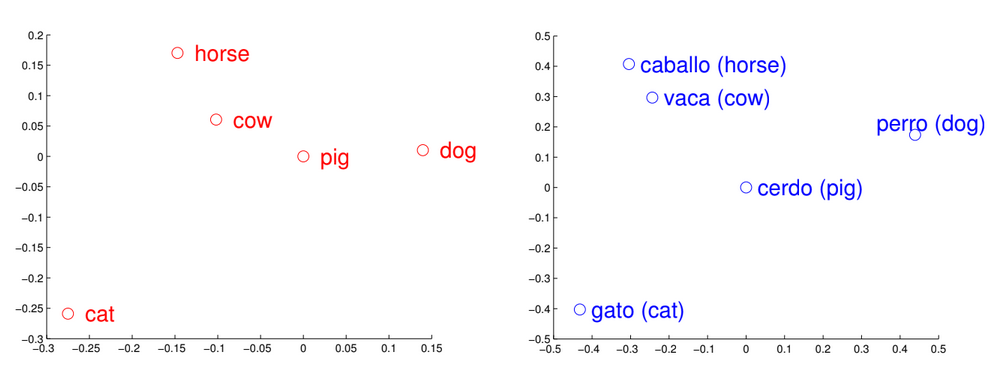
\includegraphics[width=16cm, height=8cm]{images/machine-translation.PNG}\\
\centering
\caption{Machine Translation - English to Spanish. Example showing word vectors having similar structure when trained on comparable corpora}
\label{fig:foo}
\end{figure}

\newpage
\section{Current advances in word embeddings}

Though pre-trained word embeddings have been very influential, they have a major limitation - they presume that a word's meaning is stable across sentences. However this approach to word representation does not address polysemy, or the co-existence of many possible meanings for a given word or phrase. There can be cases where there are major differences in meaning for a single word: e.g. get (a verb for obtaining) and get (an animal's offspring); or bank (a financial institution) and bank (someone to rely on). Also traditional word vectors are a single layer of weights, a shallow representation. Such word vectors fail to capture higher-level information that might be even more useful. Recent advances in NLP go from just initializing the first layer of the model to pre-training the entire model with hierarchical representations to make the model capable of performing diverse range of tasks including question answering, natural language inference etc.\\

\noindent \textbf{Embeddings from Language Models (ELMo)}\\

The motivation for ELMo \cite{peters2018deep} is that word embeddings should incorporate both word-level characteristics as well as contextual semantics. So instead of taking just the final layer of deep bi-LSTM language model as the word representation, ELMo embeddings are a function of all internal layers of bi-LSTM. The intutition is that higher level states of the bi-LSTM capture context, while lower level captures syntax. Thus, instead of using a fixed embedding for each word, ELMo looks at the entire sentence before assigning each word an embedding thus generating different embeddings for each of its occurence.

\newpage
\noindent \textbf{Open AI GPT (Generative Pre-training Transformer)}\\

Open AI GPT \cite{radford2018improving} is similar to ELMo, with a few differences. Firstly while ELMo uses Bi-LSTMs, GPT is a multi-layer encoder-decoder model with attention mechanism. Secondly while ELMo feeds embeddings into models for customized tasks, GPT fine tunes the same base model for all tasks.

However, one drawback of the GPT is its uni-directional nature - the model is only trained to predict the future left-to-right context.\\

\noindent \textbf{Bidirectional Encoder Representations from Transformers (BERT)}\\

BERT \cite{devlin2018bert} is a direct descendent to GPT — train a large language model on free text and then fine-tune on specific tasks without customized network architectures. Compared to GPT, the largest difference and improvement of BERT is to make training bi-directional. The model learns to predict both context on the left and right. The model architecture of BERT is a multi-layer bi-directional Transformer encoder.